In the prequel, we took an approach to modeling problems that evolved over time through Ordinary Differential Equations (ODEs). Though these equations were interesting in their own right, they make up but a tiny fraction of dynamical problems that scientists find interesting. Moreover, our equations typically consisted of a single dependent variable $x$ which depended on the parameter $t$ which we thought of as time. Given that we have sufficient understanding of higher dimensional spaces, it behooves us to revisit ODEs in a new light.

First, we take a cursory view of higher dimensional ODEs. The theory here will naturally lead us to the richer theory of Partial Differential Equations (PDEs). This path is actually rather direct as a handful of important PDEs can be explicitly derived from higher dimensional analogs of example ODEs we have already encountered. Once a satisfying bridge is built, we will forgo the need of explicit derivation for sake of understanding more elaborate equations that describe the fabric of nature.


\section{Higher dimensional ODEs}
        Though ODE consist of a single variable, it's possible that many ODE interact with each other and form a system.  Another case of interest would be finding trajectories as curves in higher dimensions. We may find ourselves thinking of tracking particles in space, but the components of a system need not be the same components of physical space. For example, the system could represent atmospheric dynamics along lines of latitude as in the Lorenz '96 model.
        
        For now, let us take an example with a system of two first order ODEs. In general, this assumes the form
        \begin{align}
        \label{eq:system_of_odes1}
            \dot{x}_1(t) &= f_1(x_1,x_2,t),\\
        \label{eq:system_of_odes2}
            \dot{x}_2(t) &= f_2(x_1,x_2,t).
        \end{align}
    This is an example of a first order equation with only two dependent variables, but in general we can allow for $n$ dependent variables and there is no restriction on the order of equations.
        
        \begin{df}{System of ODEs}{system_of_odes}
            A \boldgreen{system of ODEs}\index{system of ODEs} is a collection of differential equations of various order.  We call the system \boldgreen{coupled}\index{coupled} if one of the differential equations is dependent on another.
        \end{df}

        In the above equations, the coupling can be seen in each equation quite explicitly. If we set $f_1(x_1,x_2,t)=x_1+x_2$, then we can note that the $t$ derivative of $x_1$, $\dot{x}_1$, explicitly has a dependence on the current value of both $x_1$ and $x_2$. Hence, the values for $x_1$ are coupled to the other dependent variable of the system, $x_2$.
        
        \begin{ex}{SIR Model in Ecology}{sir_model}
        A biological example of a system of first order equations comes from modeling the spread of disease in a colony.  We let $S(t)$ denote the number of susceptible animals, $I(t)$ denote the number of infected animals, and $R(t)$ denote the animals resistant to the disease.  The model is a system of ODE of the form
        \begin{align*}
            \dot{S} &= -\frac{\beta IS}{N},\\
            \dot{I} &= \frac{\beta I S}{N} - \gamma I,\\
            \dot{R} &= \gamma I.
        \end{align*}
        We let $N=S(t)+I(t)+R(t)$ denote the constant population, and $\beta$ and $\gamma$ are other measured parameters. 
        
        This is a coupled system since, for example, the equation $\dot{S}$ contains the function $I$.  We also see that the equation for $\dot{I}$ contains the function $S$.  Lastly, the equation for $\dot{R}$ contains the function $I$.  
        \end{ex}

        This notation can be condensed quite readily. We can simply condense the quantities of the system, $x_1,x_2,\dots,x_n$ into a vector $\vecx$ such that
    \begin{equation}
    \label{eq:state}
        \vecx(t) = \begin{pmatrix} x_1(t) \\ x_2(t) \\ \vdots \\ x_n(t) \end{pmatrix}.
    \end{equation}
     We refer to this vector $\vecx$ as the \boldgreen{state}\index{state} of the system. Likewise, the $t$ derivative of the state is the tangent vector $\vecxdot$. The functions for the derivatives on the right hand side of  \cref{eq:system_of_odes1,eq:system_of_odes2}, $f_1,f_2,\cdots,f_n$, can also be vectorized by
\begin{equation}
    \vecf(\vecx,t) = \begin{pmatrix} f_1(\vecx,t) \\ f_2(\vecx,t) \\ \vdots \\ f_n(\vecx,t) \end{pmatrix}.
\end{equation}
This then leads to a notationally compact version of a system of differential equations by
\begin{equation}
\label{eq:first_order_system}
\vecxdot(t) = \vecf(\vecx,t).
\end{equation}
Finally, we should mention the caveat that these higher dimensional ODEs must be supplied with initial conditions in order to determine a unique curve that solves the problem at hand. We supply this as
\begin{equation}
\vecx(0)=\vecx_0,
\end{equation}
where $\vecx_0$ is some chosen vector.

One may ask about higher order systems, but truthfully all systems of ordinary differential equations can be reduced to a system of this form. This shall suffice for now. It also allows us to supply an initial condition of the state with no reference to the $t$ derivatives of the state. In higher order problems, we would also have to supply, for example, first order derivative information. Once again, we appeal to the fact that we can always describe any system as first order.


 
\section{Linear systems and flows}
        
        One special case of higher dimensional ODEs are those that are linear. Fortunately, these systems are completely solvable and well understood. We will not discuss the explicit solutions (though the reader may find them interesting) and concentrate on our bridge to PDEs.
        
        \begin{df}{Linear System of ODE}{linear_system}
            A system of first order differential equations is \boldgreen{linear}\index{linear} if it can be expressed as a matrix equation
            \[
            \vecxdot = [A(t)]\vecx,
            \]
            otherwise the system is \boldgreen{nonlinear}\index{nonlinear}. 
        \end{df}
        
        Looking back at the system in \cref{ex:sir_model}, we can note that it is nonlinear. The reason why is due to the infection terms where we see $IS$ appear. This multiplication between the dependent variables $I$ and $S$ cannot be captured through matrix multiplication. 

        \begin{ex}{Heat system}{heat_system}
        If we have three particles with temperatures $u_1,u_2$, and $u_3$ that interact with one another. We can model the system as 
        \begin{align}
        \dot{u}_1 &= -k_1 u_1 + k_1 u_2\\
        \dot{u}_2 &= -k_1 u_2 -k_2 u_2 + k_1 u_1 + k_2 u_3\\
        \dot{u}_3 &= -k_2 u_3 + k_2 u_2.
        \end{align}
        Hence, we can put
        \begin{equation}
        \boldsymbol{\dot{\vec{u}}} = [L] \boldsymbol{\vec{u}},
        \end{equation}
        where we have the matrix $[L]$ given by
        \begin{equation}
        [L] = \begin{pmatrix} -k_1 & k_1 & 0 \\ k_1 & -(k_1+k_2) & k_2 \\ 0 & k_2 & -k_2 \end{pmatrix}.
        \end{equation}
        One can see that in this system, the temperature $u_1$ depends on the temperature $u_2$, whereas the temperature $u_2$ depends on both $u_1$ and $u_2$, and finally $u_3$ depends on $u_2$. Pictorially, this would place the object 2 between the objects 1 and 3 and heat would flow between the objects in contact. The constants $k_j$ describe the ability to transport heat between the different objects. In this case, $k_1$ is the transport medium between objects 1 and 2 and $k_2$ is the transport medium between objects 2 and 3. We revisit this in more detail later.
        \end{ex}

        Vector fields play an intimate role in describing the evolutions of systems. Much of our interpretations of vector fields were given under the assumption that they describe a system in motion. For example, a vector field with divergence will cause straight line acceleration of a particle placed in the field. Curl, on the other hand, causes particles to rotate in a plane. Of course, vector fields can have both divergence and curl and the values for both can be spatially dependent. To complete this description, we provide the following definition.

        \begin{df}{Flow}{flow}
        Let $\vecx$ be the state of a system in $\R^n$ and let $\vecfieldV$ be an $n$-dimensional vector field. Then the \boldgreen{flow of the vector field $\vecfieldV$} is
    \begin{equation}
    \vecxdot(t)= \vecfieldV(\vecx(t)).
    \end{equation}
        \end{df}

        The interpretation here is that the tangent vector of the curve is equal to the vector field at all points in time $t$ so that the curve follows the vector field. In principle, the vector field $\vecfieldV$ could also depend on the variable $t$ explicitly for which we would arrive at an equation of the form \cref{eq:first_order_system}. This would happen when, for example, if the wind in a region changes over time, we would have both spatial dependence from $\vecx$ and time dependence from $t$ so that we must put $\vecf(\vecx,t)$.

        \begin{ex}{Helical flow}{helical_flow}
        Consider the vector field $\vecfieldV=\begin{pmatrix} -y \\ x \\ \frac{1}{4}z \end{pmatrix}$. Note that
    \begin{align}
    \grad \times \vecfieldV = \begin{pmatrix} 0 \\ 0 \\ 2 \end{pmatrix}\\
    \grad \cdot \vecfieldV = \frac{1}{10}.
    \end{align}
    Hence, we should expect rotation in a plane except when $x=y=0$ along with acceleration in a straight line at any point in space aside from where $z=0$. To this end, we consider the initial value problem for the flow of $\vecfieldV$ by
    \begin{equation}
    \vecxdot = \vecfieldV(\vecx) \qquad \vecx(0)=\begin{pmatrix} 1 \\ 0 \\ \frac{1}{2} \end{pmatrix}.
    \end{equation}
    The above equation is also linear since it can be written in terms of a matrix. This makes it possible to find a close form analytical solution. We note the solution to the initial value problem is
    \begin{equation}
    \vecx(t) = \begin{pmatrix} \cos(t) \\ \sin(t) \\ \frac{1}{2}e^{\frac{t}{4}} \end{pmatrix}.
    \end{equation}
    In general, it may only be possible to approximate a solution computationally, but this is a rather quick task as well. Let us view this solution along with the vector field.
    \begin{figure}[H]
     \centering
     \begin{subfigure}[b]{0.3\textwidth}
         \centering
         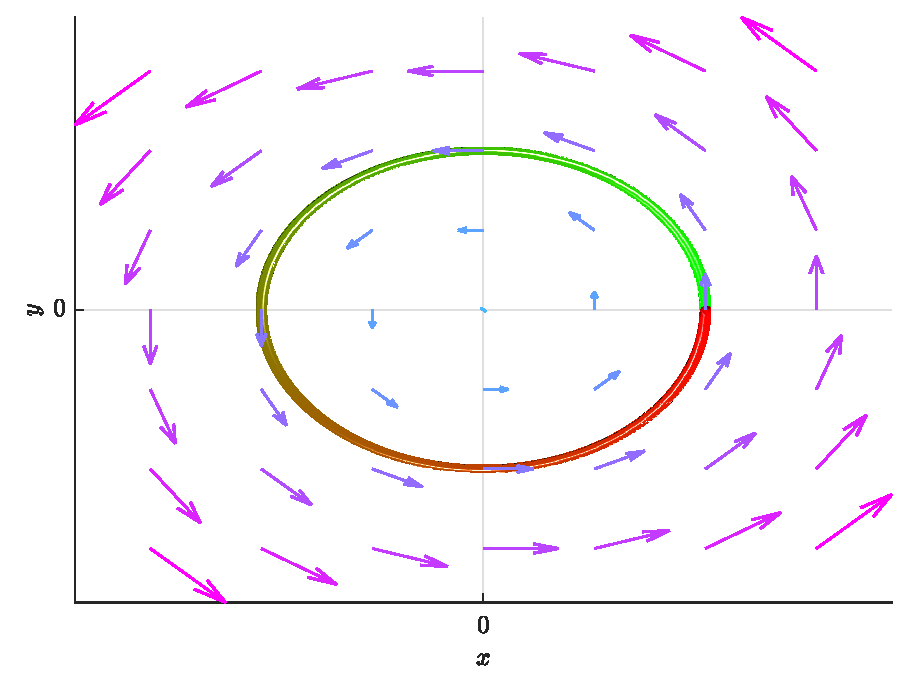
\includegraphics[width=\textwidth]{Figures_Part_6/flow_xy}
         \caption{Looking towards $xy$-plane.}
         \label{fig:flow_xy}
     \end{subfigure}
     \hfill
     \begin{subfigure}[b]{0.3\textwidth}
         \centering
         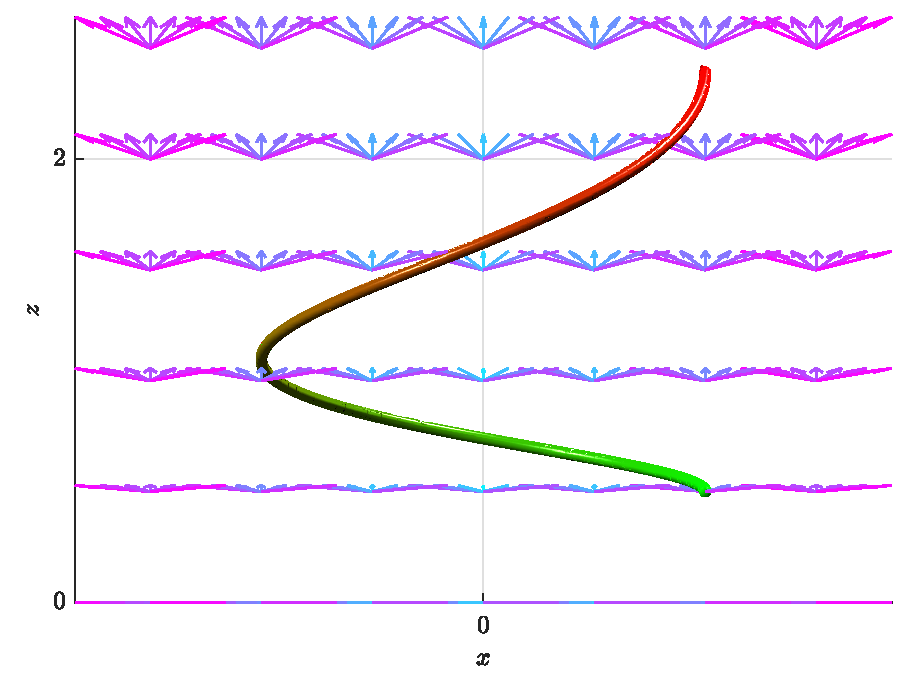
\includegraphics[width=\textwidth]{Figures_Part_6/flow_xz}
         \caption{Looking towards $xz$-plane.}
         \label{fig:flow_xz}
     \end{subfigure}
     \hfill
     \begin{subfigure}[b]{0.3\textwidth}
         \centering
         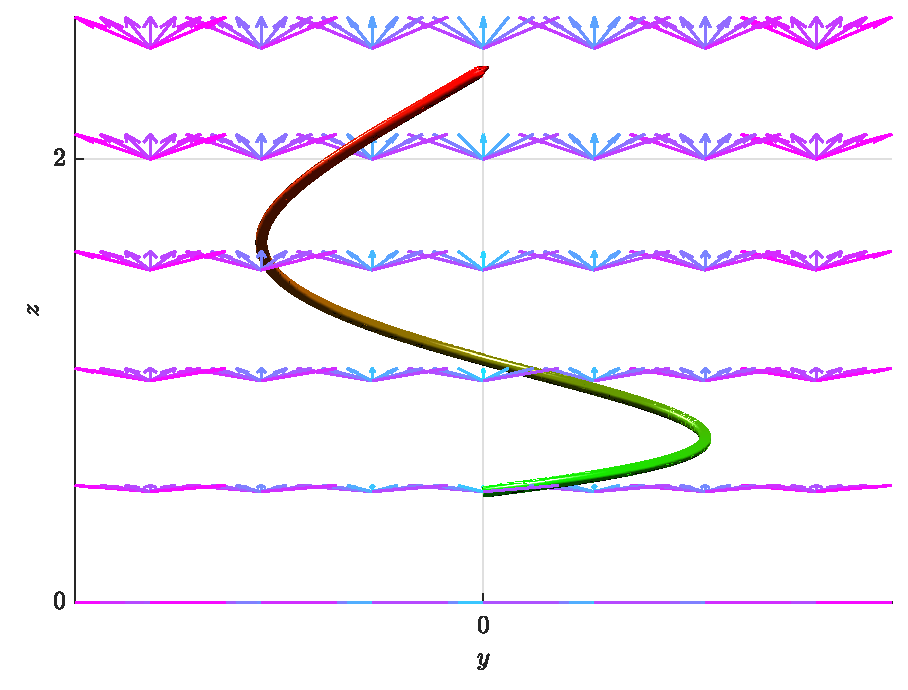
\includegraphics[width=\textwidth]{Figures_Part_6/flow_yz}
         \caption{Looking towards $yz$-plane.}
         \label{fig:flow_yz}
     \end{subfigure}
        \caption{The curve $\vecx$ and the vector field $\vecfieldV$ from different angles.}
        \label{fig:flow}
\end{figure}
        \end{ex}

\begin{exercise}
    Show that \cref{ex:helical_flow} is linear by constructing a matrix $[A]$ such that $\vecxdot = [A]\vecx$.
\end{exercise}

        One other interesting and widely applicable type of systems are the gradient systems. These systems are used to describe physical processes such as fluid flow or heat flow. Not only that, but for problems where one is seeking to find a minimal or optimal solution, one can use a gradient system as a means of approaching the optimum. In particular, this method is used in machine learning in the gradient descent algorithm. 

        \begin{df}{Gradient flow}{gradient_flow}
        Let $\vecx$ be the state of a system in $\R^n$ and let $f\colon \R^n \to \R$ be a scalar field. Then the flow 
        \begin{equation}
        \vecxdot(t) = \grad f(\vecx(t))
        \end{equation}
        is called \boldgreen{gradient flow} \index{gradient!flow}.
        \end{df}

        The interpretation of a gradient flow is that the state tends towards a local maximum of the function $f$. If we took the flow defined by the negative of the gradient
\begin{equation}
    \vecxdot(t) = -\grad f(\vecx(t)),
\end{equation}
then the state would tend towards the local minimum value of of $f$. This is sometimes referred to as \boldgreen{gradient descent}\index{gradient!descent}. Examples of physical scenarios involving gradient descent include fluid dynamics and heat transfer.
        
    \section{Partial Differential Equations}

        We now want to investigate a larger class of differential equations.  These are the \boldgreen{partial differential equations} (PDEs).  These equations become yet more complicated to solve, but are very prevalent in the study of the physical world. Fundamentally, these are time-varying differential equations of vector and scalar fields of many variables.  The goal for us is to be able to recognize a few specific example equations and understand their behavior.  We will also be able to solve a few equations with our tools from studying ODEs. However, it is easy to pose a PDE that is virtually impossible to solve.  
        
        \begin{df}{Scalar Partial Differential Equation}{pde}
        A \boldgreen{partial differential equation of a scalar field} of three spatial variables $x,y,z$ and a time variable $t$ is an expression of a scalar function $u(x,y,z,t)$, the partial derivatives of $u(x,y,z,t)$, and other functions.
        \end{df}
        
        \begin{df}{Vector Partial Differential Equation}{vec_pde}
        A \boldgreen{partial differential equation of a vector field}
        \[
        \vecfieldV(x,y,z,t) = \begin{bmatrix} V_1(x,y,z,t) \\ V_2(x,y,z,t) \\ V_3(x,y,z,t) \end{bmatrix}
        \]
        is an equation containing $\vecfieldV$, the (component) derivatives of $\vecfieldV$, and other vector fields.
        \end{df}
        
        It is worthwhile to take a look at a few important example equations before we move onto derivations or methods of solutions. The realms of PDEs are so widespread, it is rather difficult to give a comprehensive list. It is even difficult to list the applications of a single equation. To begin, we will consider three intimately related scalar equations. Each of which, we will derive in some way. Finally, we list the vector equations for the laws of electrodynamics and the time dependent Schr\"odinger equation.

        
        \begin{ex}{Heat equation}{heat_eqn}
        The scalar \boldgreen{heat equation} is given by
        \begin{equation}
        \label{eq:heat_eqn}
        \frac{\partial u}{\partial t}(\vecx,t) -\grad \cdot (k(\vecx)\grad u(\vecx,t)) = f(\vecx,t),
        \end{equation}
        where $\vecx$ represents a position in space (typically $\R^3$). This equation models the diffusion of heat in a region of space, hence the name. We think of $u(\vecx,t)$ being the temperature at the point $\vecx$ at the time $t$.
        \end{ex}
        
        \begin{ex}{Laplace (Poisson) equation}{laplace}
        The scalar \boldgreen{Laplace} (sometimes \boldgreen{Poisson}) \boldgreen{equation} is given by
        \begin{equation}
        \label{eq:laplace_eqn}
        -\Delta u(\vecx) = f(\vecx).
        \end{equation}
        Notice, there is no dependence on time! This equation can be realized as the long term behavior of the heat equation.  If $u(\vecx)$ describes temperature, then the solution to this equation tells you the equilibrium temperature. Since this is an equilibrium solution, the time component is gone.
        \end{ex}
        
        \begin{ex}{Wave equation}{wave}
        The scalar \boldgreen{wave equation} is given by
        \begin{equation}
        \label{eq:wave_eqn}
        \frac{\partial^2 u}{\partial t^2}(\vecx,t) -c^2\Delta u(\vecx,t) = f(\vecx,t).
        \end{equation}
        The solutions here are wavelike.  Think of plucking a guitar string, or the ripples on the surface of a lake after a rock has been tossed in, or the vibrating cymbal or drum head.
        \end{ex}
        
        \begin{ex}{Maxwell's equations}{maxwell}
        Maxwell's equations describe the electric $\vecfieldE$ and magnetic $\vecfieldB$ fields that permeate space due to charged particles.  These equations turn out to be coupled PDE.  They read
        \begin{align}
            \grad \cdot \vecfieldE(\vecx,t) &= \frac{\rho(\vecx,t)}{\epsilon},\\
            \grad \cdot \vecfieldB(\vecx,t) &= 0,\\
            \grad \times \vecfieldE(\vecx,t) &= -\frac{\partial \vecfieldB}{\partial t}(\vecx,t),\\
            \grad \times \vecfieldB(\vecx,t) &= \mu \vecfieldJ + \mu \epsilon \frac{\partial \vecfieldE}{\partial t}(\vecx,t).
        \end{align}
        The equations above are best realized when studying spacetime as a single entity. We will not cover this in this text, but one can find that electrodynamics is a rich subject deeply imbued into the fabric of the cosmos.
        \end{ex}

        \begin{ex}{Time dependent Schr\"odinger equation}{schrodinger}
        The time dependent Schr\"odinger equation models the state of a quantum system and its evolution in time. Succinctly, one sees this equation written in terms of operators by
\begin{equation}
\label{eq:schrodinger_operator_eqn}
H \Psi(\vecx,t) = E \Psi(\vecx,t),
\end{equation}
  where $H$ is the Hamiltonian operator given by
\begin{equation}
-\frac{\hbar^2}{2m} \Delta + V(\vecx)
\end{equation}
and $E$ is the energy operator given by
        \begin{equation}
i\hbar \frac{\partial}{\partial t}.
\end{equation}
Hence, we have
\begin{equation}
\label{eq:schrodinger_time}
\left(-\frac{\hbar^2}{2m} \Delta + V(\vecx)\right) \Psi(\vecx,t) = i\hbar \frac{\partial}{\partial t} \Psi(\vecx,t)
\end{equation}
We will return to this equation in more depth later.
        \end{ex}
       
    
    % %%%%%%%%%%%%%%%%%%%%%%%%%%%%%%%%%%%%%%%%%%%%%%%%%%%%%%%%%%%%%%%%%%%%%%%%%%%%%%%%%%%%
    % The Heat Equation
    % %%%%%%%%%%%%%%%%%%%%%%%%%%%%%%%%%%%%%%%%%%%%%%%%%%%%%%%%%%%%%%%%%%%%%%%%%%%%%%%%%%%%
    
        \section{The heat equation}
        
        Imagine at this moment, that we are to generalize \cref{ex:heat_system} to a system with $n$ particles. If we then take the limit as $n \to \infty$, we should expect nothing less than to arrive at the heat equation we see in \cref{ex:heat_eqn} with the caveat that we would be taking a 1-dimensional approach. Keep this in mind as we proceed -- you know where we are starting and where we are heading. Let us now explicitly consider this scenario. Let us imagine a rod lined with $n$ equally particles spaced particles with a heat conductive medium placed between the interior particles. This gives us the following picture.
\begin{figure}[H]
	\centering
	\resizebox{\columnwidth}{!}{\input{Figures_Part_6/equally_spaced_line_points.pdf_tex}}
\end{figure}
        We label the position of the $j^\textrm{th}$ particle as $x_j$ and the thermally conductive media between particle $j$ and $j+1$ will be given a value of $k_j$. The value of $k_j$ describes how easily thermal energy is transported between particle $j$ and $j+1$. Larger $k_j$ means more heat can be transferred at any given moment. $k_j$ can be referred to as the \boldgreen{diffusivity}\index{diffusivity} of the thermal transport medium. We then let $u(x,t)$ be the temperature at the point $x$ and time $t$ along the rod. For now, we will define $u$ only on the particles and note that we will put $u(x_j,t)=u_j(t)$. We can place additional sources of heat on each particle by taking a function $f(x,t)$ and defining $f_j(t) \coloneqq f(x_j,t)$. The function $f(x,t)$ describes the rate of thermal energy added at the point $x$ at the time $t$.
    \begin{exercise}
    Run a thought experiment in your head. Pick a small value of $n$, choose some temperatures $u_j$ for all of particles, and ignore the heat sources $f_j$ for the time being. What do you think will happen as time moves forward?
    \end{exercise} 
        In this rod, we can refer to the endpoints $x_1$ and $x_n$ as the boundaries and the other $n-2$ points as the interior. Let us deduce the equations for the boundary and interior. First, particle 1 radiates heat through the medium $k_1$ while particle 2 does the same. This process is random, but on average, we find that the rate of change of temperature of particle 1 depends on how much is lost and gained in the interaction with particle 2. The law of mass action then states
    \begin{equation}
        \dot{u}_1 = -k_1 u_1 + k_1 u_2 + f_1= k_1(u_2-u_1)+f_1.
    \end{equation}
        The second equality shows that this is equivalent Newton's law of cooling with an additional source of heat from the rate due to $f$! The equation for particle $n$ follows a completely analogous argument and we have
\begin{equation}
    \dot{u}_n = -k_{n-1} u_n + k_{n-1} u_{n-1} + f_n.
\end{equation}
        The interior points are only more complicated in the sense that each has two neighbors. The interior particle $j$ will interact with both particles $j-1$ and $j+1$ by
 \begin{equation}
\dot{u}_j = -k_{j-1} u_j - k_j u_j + k_{j-1} u_{j-1} + k_j u_{j+1} + f_j = k_j (u_{j+1}-u_j) - k_{j-1}(u_j-u_{j-1}) + f_j.
\end{equation}
Since this process of heat is random, we can imagine that quanta of heat are passed between the particles and so, if the rod has a conductivity $\kappa$, then $k = \frac{\kappa}{\delta x^2}$ will describe how much heat flow between any two particles. Here, $\delta x$ is the distance between any two particles (i.e., $\delta x = x_j-x_{j-1}$). This is due to the fact that, on average, a quanta of heat will travel a distance proportional to $\delta x^2$. Hence, we shall replace the instances of $k_j$ with $\frac{\kappa_j}{\delta x^2}$ where and we have
\begin{equation}
\dot{u}_j = \frac{ \kappa_j (u_{j+1}-u_j) - \kappa_{j-1}(u_j-u_{j-1})}{\delta x^2} + f_j.
\end{equation}
If we now take the limit that $n\to \infty$, then $\delta x \to 0$ and we have for interior points $x\in (x_1,x_n)$
\begin{equation}
\frac{\partial}{\partial t} u(x,t) = \frac{\partial}{\partial x} \left( \kappa(x) \frac{\partial}{\partial x} u(x,t)\right) + f(x,t).
\end{equation}
One should now compare this equation to that in \cref{ex:heat_eqn} in the case where the spatial dimension is equal to one.

        
\textcolor{red}{Stopped updating here. Mention gradient flows and linear systems. Write the above as a linear system?}
        
        One of the most illuminating examples of PDEs is the heat equation.  Let us work through a specific example of the heat equation and keep in mind the physical intuition throughout.
        
        In order to move forward, we need to also properly specify the problem we want to solve.
        
        The one-dimensional source-free heat equation is a great starting point to begin our process.  We are given the following data:
        \begin{itemize}
            \item A region $\Omega$ in space that we are concerned with.  For example, in one dimension, we can consider the interval $\Omega=(0,1)$.
            \item A PDE
            \[
            \frac{\partial u}{\partial t}(x,t) -k \frac{\partial^2 u}{\partial x}^2 = 0.
            \]
            \item Boundary conditions. These can come in a few forms, but we will concentrate on just one. We must specify $u(0,t)=a$ and $u(1,t)=b$.  These boundary conditions correspond to fixing the temperature at the ends of a rod constant.
            \item Initial conditions. We specify the initial temperature distribution
            \[
            u(x,0)=u_0(x).
            \]
        \end{itemize}

        \begin{ex}{Solving the Heat Equation}{solving_heat_equation}
        Let us consider the simplified one-dimensional source free (i.e., the right hand side is zero) heat equation given by the following:
        \[
        \frac{\partial u}{\partial t}(x,t)-\frac{\partial^2 u}{\partial x^2} = 0.
        \]
        We can require boundary conditions and initial conditions later on.\\
        
        Let us assume that the solution function $u(x,t)$ can be written as
        \[
        u(x,t) = f(x)g(t).
        \]
        We call this approach the \boldgreen{separation of variables}. We then plug in this assumption to our PDE.
        \begin{align*}
            \frac{\partial}{\partial t} (f(x)g(t))-\frac{\partial^2}{\partial x^2} (f(x)g(t)) &= 0\\
            f(x)\frac{\partial g}{\partial t}-g(t)\frac{\partial^2 f}{\partial x^2}&=0\\
            fg'-f''g &=0.
        \end{align*}
        We can then do a bit more algebra.
        \begin{align*}
            fg'-f''g&=0\\
            fg'&= f''g\\
            \frac{g'(t)}{g(t)}&=\frac{f''(x)}{f(x)}.
        \end{align*}
        Now, notice that both sides depend on different variables.  We have successfully separated this equation into an equation for each variable.  This is to say, since each side of the equation depends on a different variable, each side must be equal to a constant $\lambda$! So we have two equations.
        \begin{align*}
            \frac{g'(t)}{g(t)}&=\lambda\\
            \frac{f''(x)}{f(x)}&=\lambda.
        \end{align*}
        We can then solve both of these as ODE. Note, it will be helpful to to instead choose $-\lambda$ as the constant.
        \end{ex}
        
        \begin{exercise}
        What are the general solutions to the above ODE?
        \end{exercise}
        
        \begin{exercise}
        Given those general solutions, what is the general solution to the heat equation?
        \end{exercise}
        
        \begin{answer}
        We get
        \[
        \boxed{u(x,t)=f(x)g(t) = Ae^{-\lambda y}\sin(\sqrt{\lambda}x)+Be^{-\lambda t}\cos(\sqrt{\lambda}x).}
        \]
        \end{answer}
        
        Previously we found the general solution to the heat equation 
        \[
        \frac{\partial u}{\partial t}(x,t) - \frac{\partial^2 u}{\partial x^2} (x,t) = 0
        \]
        is
        \[
        u(x,t)=Ae^{-\lambda t}\sin(\sqrt{\lambda}x)+Be^{-\lambda t}\cos(\sqrt{\lambda}x).
        \]
        However, this solution is very general.  We have the undetermined constants $\lambda$, $A$, and $B$. We need more information to get a particular solution.
        
        \begin{ex}{Particular Solution to the 1D Heat Equation}{particular_heat}
        We will stick with the one-dimensional case but we must pick the following.  
        \begin{itemize}
            \item Domain: Let $\Omega = (0,1)$.
            \item Initial Conditions: $u(x,0)=\sin(\pi x)$.
            \item Boundary Conditions: $u(1,t)=u(0,t)=0$.  
        \end{itemize}
        This list of requirements gives us enough information to solve the equation explicitly for a particular solution.\\
        
        First, let us take the boundary conditions. We impose these on our general solution:
        \[
        u(x,t)=Ae^{-\lambda t}\sin(\sqrt{\lambda}x)+Be^{-\lambda t}\cos(\sqrt{\lambda}x).
        \]
        Thus we require
        \[
        0=u(0,t)=Ae^{-\lambda t}\sin(0)+Be^{-\lambda t}\cos(0)
        \]
        which gives us that
        \[
        B=0.
        \]
        The other boundary condition is
        \[
        0=u(1,t)=Ae^{-\lambda t}\sin(\sqrt{\lambda}).
        \]
        Specifically, this means that $A=0$, which gives us a trivial solution or that we have
        \[
        \sqrt{\lambda}=n\pi
        \]
        for any integer $n$.  This is because $\sin(n\pi)=0$ when $n$ is an integer. Thus our solution now reads
        \[
        u(x,t)=Ae^{-n^2\pi^2}\sin(n\pi x).
        \]
        
        Lastly, we match our initial conditions.  So we have
        \[
        \sin(\pi x)=u(x,0)=A e^0 \sin(n\pi x)
        \]
        and so we find that $n=1$.  Thus, our solution is
        \[
        \boxed{u(x,t)=e^{-\pi^2 t} \sin(\pi x).}
        \] 
        
        We can plot this solution as follows.
        \begin{figure}[H]
        	\centering
        	\def\svgwidth{0.75\columnwidth}
        	\input{Figures_Part_7/heat_solution.pdf_tex}
        \end{figure}
        \end{ex}
        
        \begin{exercise}
        Can you interpret what this is physically describing as $t$ gets larger?
        \end{exercise}
        
    % %%%%%%%%%%%%%%%%%%%%%%%%%%%%%%%%%%%%%%%%%%%%%%%%%%%%%%%%%%%%%%%%%%%%%%%%%%%%%%%%%%%%
    % The Laplace Equation
    % %%%%%%%%%%%%%%%%%%%%%%%%%%%%%%%%%%%%%%%%%%%%%%%%%%%%%%%%%%%%%%%%%%%%%%%%%%%%%%%%%%%%
    
        \section{The Laplace Equation}
        In the long time limit ($t\to \infty$) or steady-state of the (source free) heat equation, one arrives at the so called Laplace equation
        \[
        -\Delta u = 0.
        \]
        In the one-dimensional case, this equation reads
        \[
        -\frac{d^2 u}{dx^2}(x) = 0.
        \]
        Note there is no dependence on time as this is the steady-state behavior for the heat equation.
        
        \begin{exercise}
        This is an ODE in the variable $x$.  You can solve this and find a general solution by integration.  
        \end{exercise} 
        
        \begin{answer}
        The general solution to the one-dimensional Laplace equation is the equation for a line
        \[
        u(x) = Ax+B.
        \]
        One can show that this is indeed a solution by taking two derivatives of $u(x)$ and finding that you get zero.
        \end{answer}
        
        \begin{ex}{Particular Solution to the 1D Laplace Equation}{particular_laplace}
        Through integration, we find
        \[
        u(x) = Ax+B
        \]
        where $A$ and $B$ are undetermined constants.  In order to specify these constants, we must provide the following.
        \begin{itemize}
            \item Domain: Let $\Omega = (0,1)$.
            \item Boundary Conditions: $u(0)=0$ and $u(1)=0$.  
        \end{itemize}
        Note that we do not need initial conditions since there is no time dependence in this PDE.\\
        
        Now, to find the particular solution, we apply the boundary conditions to our general solution.  So we have
        \[
        0=u(0)=A(0)+B,
        \]
        so $B=0$.  Then the other condition 
        \[
        0=u(1)=A,
        \]
        so $A=0$.  Thus, our solution is
        \[
        \boxed{u(x)=0}.
        \]
        Now, compare this to the solution to the heat equation previously
        \[
        u(x,t)=e^{-\pi^2 t}\sin(\pi x).
        \]
        We claimed the Laplace equation is the long-time solution of the heat equation and indeed if we look at $t\to\infty$, we have
        \[
        \lim_{t\to \infty} u(x,t)=0.
        \]
        \end{ex}
        
    % %%%%%%%%%%%%%%%%%%%%%%%%%%%%%%%%%%%%%%%%%%%%%%%%%%%%%%%%%%%%%%%%%%%%%%%%%%%%%%%%%%%%
    % The Wave Equation
    % %%%%%%%%%%%%%%%%%%%%%%%%%%%%%%%%%%%%%%%%%%%%%%%%%%%%%%%%%%%%%%%%%%%%%%%%%%%%%%%%%%%%

        \section{The Wave Equation}
        The wave equation is studied when one wants to find the oscillatory behavior of some medium.  For example, one can pluck a guitar string or hit a drum head.  These actions induce vibrations in the medium (the string or head) and it is the vibrations that one hears.  The equation that models these phenomenon is the wave equation
        \[
        \frac{\partial^2 u}{\partial t^2}(x,y,z,t)-c^2 \nabla \cdot \nabla u(x,y,z,t)=f(x,y,z,t).
        \]
        
        \begin{ex}{Solving the 1D Wave Equation}{1d_wave}
        In one-dimension, the simplified source free wave equation reads
        \[
        \frac{\partial^2 u}{\partial t^2}(x,t) -\frac{\partial^2 u}{\partial x^2}(x,t)=0.
        \]
        
        It turns out we can solve the 1D wave equation in the same way we did the heat equation. So, we assume a separation of variables approach in that 
        \[
        u(x,t) = f(x)g(t).
        \]
        We plug this into the PDE to find
        \begin{align*}
            \frac{\partial^2}{\partial t^2}(f(x)g(t))-\frac{\partial^2}{\partial x^2}(f(x)g(t))&=0\\
            f(x)\frac{\partial^2 g}{\partial t^2}-g(t)\frac{\partial^2 f}{\partial x^2}&=0\\
            f(x)g''(t)-f''(x)g(t)&=0.
        \end{align*}
        We then wish to make the left hand side and right hand side functions of different input variables
        \begin{align*}
            f(x)g''(t)-f''(x)g(t)&=0\\
            f(x)g''(t)&=f''(x)g(t)\\
            \frac{g''(t)}{g(t)}&= \frac{f''(x)}{f(x)}.
        \end{align*}
        Since each side depends on a different input variable, each side must be equal to a constant.  So this gives us
        \[
        \frac{g''(t)}{g(t)}= \frac{f''(x)}{f(x)}= -\lambda^2,
        \]
        where $-\lambda^2$ is an undetermined constant but was chosen to make the next steps easier. We then get two ODEs
        \begin{align*}
            f''(x)&=-\lambda^2 f(x),\\
            g''(t)&=-\lambda^2 g(t),
        \end{align*}
        which are both harmonic oscillator equations.  Thus, since we know the solutions to the harmonic oscillator equation, we have
        \begin{align*}
            f(x)&=C_1 \sin(\lambda x)+ C_2 \cos(\lambda x),\\
            g(t)&=C_3 \sin(\lambda t)+ C_3 \cos(\lambda t).
        \end{align*}
        It follows that our solution is thus
        \[
        \boxed{u(x,t)=f(x)g(t)= (C_1 \sin(\lambda x)+ C_2 \cos(\lambda x))(C_3 \sin(\lambda t)+ C_3 \cos(\lambda t)).}
        \]
        \end{ex}
        
        With a general solution to the wave equation written down.  We can work to solve a particular case of the wave equation.  Let's see this.
        
        \begin{ex}{Particular Solution to the 1D Wave Equation}{part_wave}
        We found that the general solution to the 1D wave equation is
        \[
        u(x,t)=(C_1 \sin(\lambda x)+ C_2 \cos(\lambda x))(C_3 \sin(\lambda t)+ C_3 \cos(\lambda t)).
        \]
        Let us multiply this out and re-collect the constants to get
        \[
        u(x,t) = C_1 \sin(\lambda x)\sin(\lambda t) + C_2 \sin(\lambda x)\cos(\lambda t) + C_3 \cos(\lambda x)\sin(\lambda t)+ C_4 \cos(\lambda x)\sin(\lambda t).
        \]
        In order to specify these constants, we provide the following:
        \begin{itemize}
            \item Domain: Let $\Omega=(0,1)$.
            \item Initial Conditions: We let $u(x,0)=\sin(\pi x)$ and $\frac{\partial u}{\partial t}(x,0)=0.$ 
            \item Boundary Conditions: Take $u(0)=u(1)=0$.
        \end{itemize}
        Note the need for both initial position $u(x,0)$ and initial velocity $\frac{\partial u}{\partial t}(x,0)$.\\
        
        Now, we find the particular solution by first applying our boundary conditions.  Specifically, we have
        \[
        0=u(0,t)= C_1 \sin(0)\sin(\lambda t) + C_2 \sin(0)\cos(\lambda t) + C_3 \cos(0)\sin(\lambda t)+ C_4 \cos(0)\sin(\lambda t) 
        \]
        which reduces to
        \[
        0= C_3 \sin(\lambda t)+ C_4 \cos(\lambda t).
        \]
        The only way this can be equal to zero for all $t$ is if $C_3=C_4=0$.  Thus, we now have
        \[
        u(x,t) = C_1 \sin(\lambda x)\sin(\lambda t) + C_2 \sin(\lambda x)\cos(\lambda t).
        \]
        Applying the next boundary condition
        \[
        0=u(1,t)= C_1 \sin(\lambda ) \sin(\lambda t) + C_2 \sin(\lambda)\cos(\lambda t)
        \]
        gives us that $\lambda = n\pi$ for any integer $n$ since in this case $\sin(n\pi)=0$. And so our solution is now
        \[
        u(x,t) = C_1 \sin(n \pi x) \sin(n \pi t) + C_2 \sin(n \pi x)\cos (n \pi t).
        \]
        
        We then apply the initial conditions. Specifically, we required that
        \[
        \sin(\pi x) = u(x,0) = C_1 \sin(n\pi x) \sin(0)+ C_2 \sin(n\pi x) \cos(0)
        \]
        which reduces to
        \[
        \sin(\pi x) = C_2 \sin(n\pi x).
        \]
        Thus we have that $n=1$ and $C_2=1$.  Our solution is now
        \[
        u(x,t)=C_1 \sin(\pi x)\sin(\pi t) +  \sin(\pi x)\cos(\pi t).
        \]
        Now, we also required that
        \[
        0=\frac{\partial u}{\partial t}(x,0) =C_1 \pi \sin(\pi x)\cos(0) - \pi \sin(\pi x) \sin(0)
        \]
        which reduces to
        \[
        0 = C_1 \pi \sin(\pi x)
        \]
        which means that
        \[
        C_1=0.
        \]
        Thus, we now have the particular solution
        \[
        \boxed{u(x,t)=\sin(\pi x)\cos(\pi t).}
        \]
        We can plot a graph of this solution with $z$ representing the height of the function, the $x$-axis giving our position in the domain $\Omega$ and the $t$-axis moving perpendicularly to $x$ and $z$. We get
\begin{figure}[H]
	\centering
	\def\svgwidth{0.75\columnwidth}
	\input{Figures_Part_7/wave_solution.pdf_tex}
\end{figure}
        % \begin{figure}[H]
        %     \centering
        %     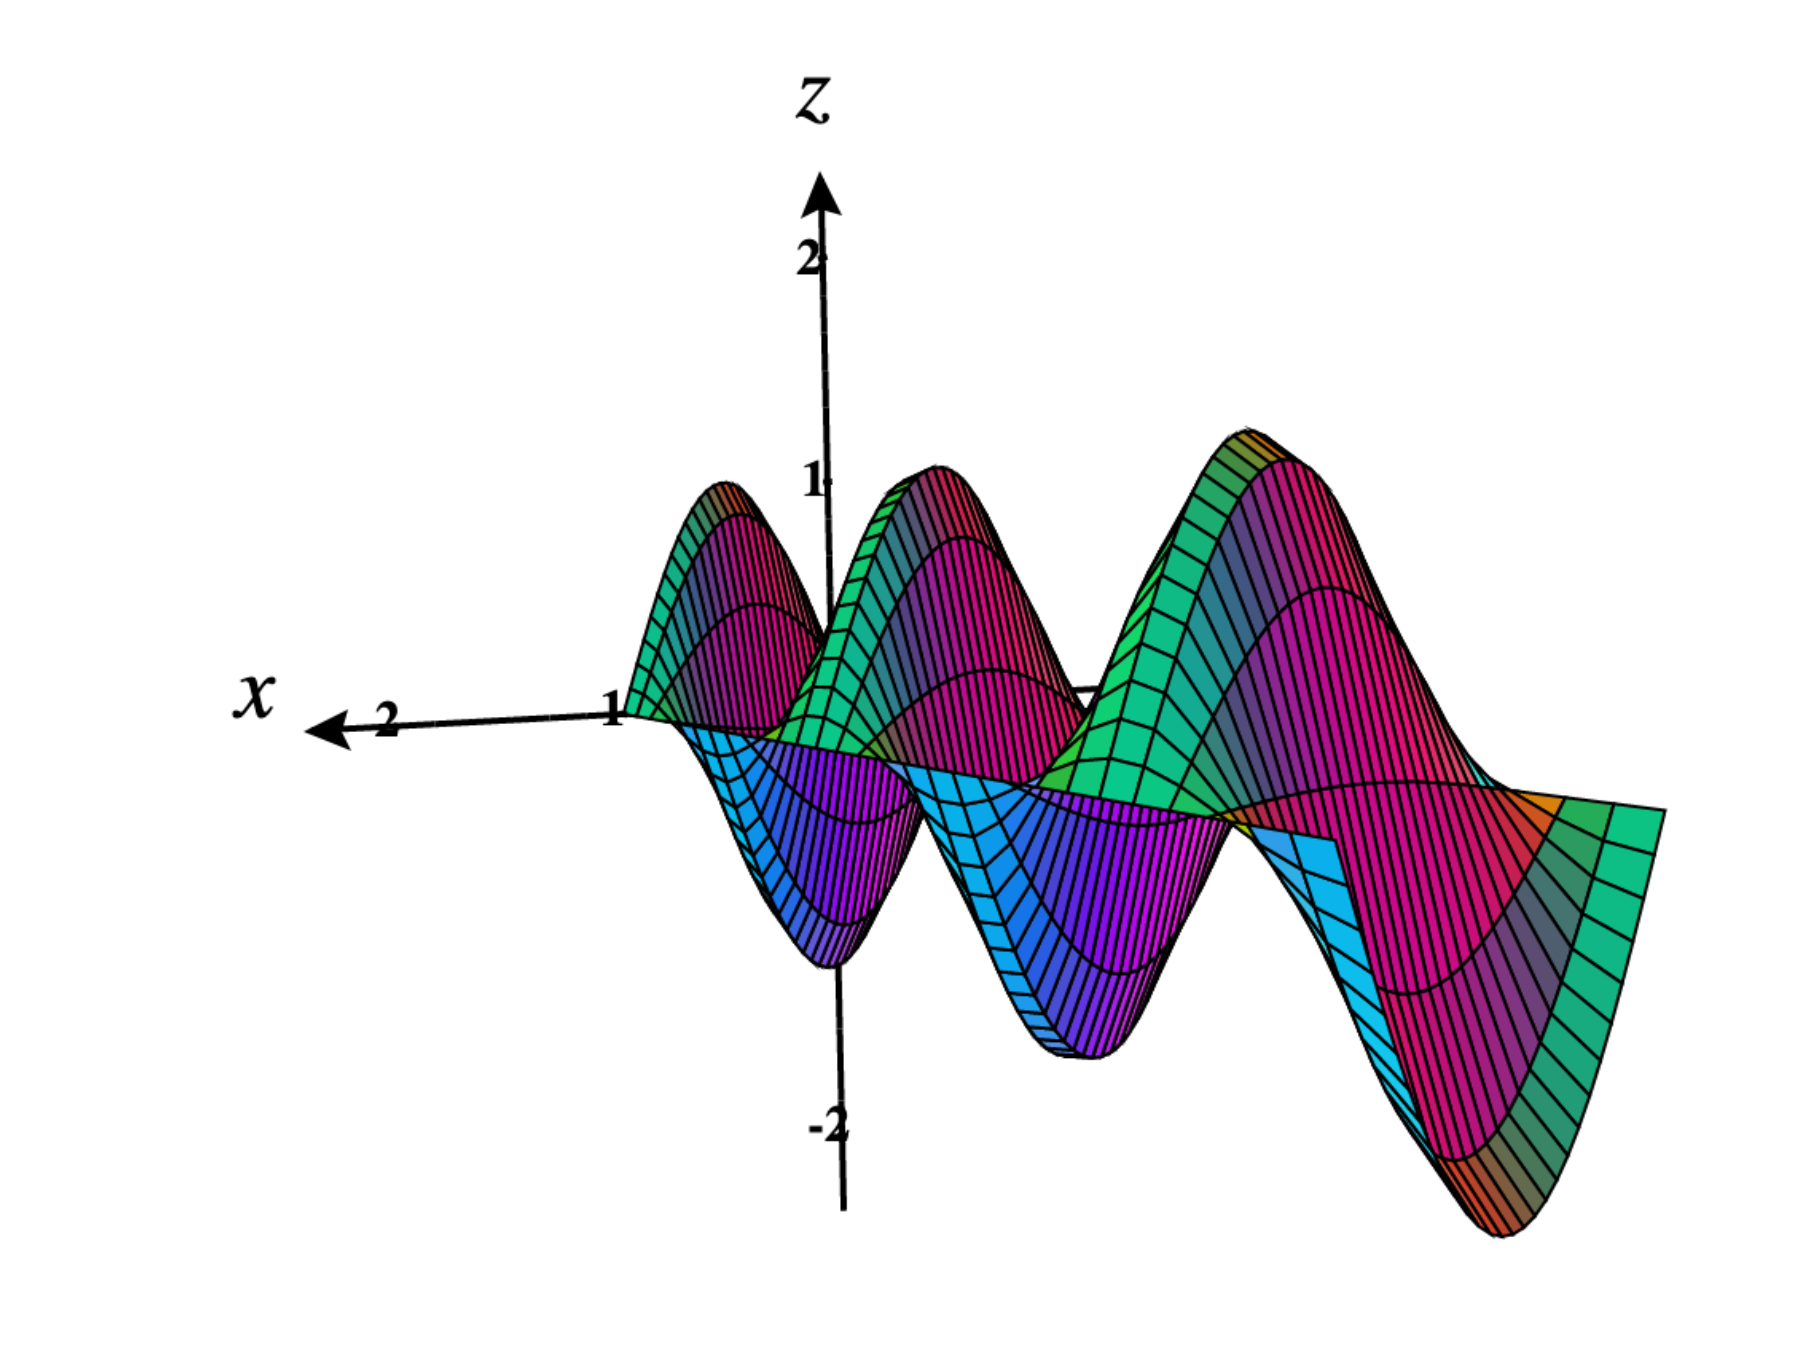
\includegraphics[width=.5\textwidth]{Figures/wave_solution.png}
        % \end{figure}
        \end{ex}

% \end{document}
